%%=============================================================================
%% Ontwerp
%%=============================================================================

\chapter{Ontwerp van de applicatie}%
\label{ch:ontwerp}

Dit hoofdstuk beschrijft de ontwerpkeuzes die gemaakt werden bij het
ontwikkelen van het prototype \textit{Flow}. De keuzes zijn gebaseerd op drie
opeenvolgende onderzoeksfasen: de literatuurstudie en vergelijkende app-analyse,
de twee semigestructureerde interviews, en de kwantitatieve survey bij 32
respondenten. Waar de eerste twee fasen de ontwerpprincipes definieerden, stuurde
de survey een aantal van deze keuzes bij in een tweede iteratie van het prototype.

\section{Ontwerpprincipes}

Op basis van de literatuurstudie, de interviewresultaten en de surveydata werden
zeven ontwerpprincipes gehanteerd.

\textbf{Lage initiatiefdrempel.}
Taken worden ingevoerd via een gestructureerd formulier of vrije tekstinvoer,
zonder verplichte structuur vooraf. Respondent~1 omschreef bestaande apps als te
arbeidsintensief in verhouding tot hun nut: \textit{``heel veel van die apps zijn
redelijk veel werk om de informatie in te geven, terwijl het niet veel return on
investment geeft''}. De survey bevestigde dit kwantitatief: 68,8\% van de
respondenten noemde een hoge invoerdrempel als absolute dealbreaker. De applicatie
verlaagt deze drempel door structuur pas ná de invoer te genereren en de
gestructureerde invoer als standaard aan te bieden, met vrij typen als
alternatief.

\textbf{Passieve zichtbaarheid boven actieve notificaties.}
Beide respondenten gaven aan dat notificaties reflexmatig worden weggeklikt.
Respondent~2 verkoos widgets op het startscherm: \textit{``als dat op je
startscherm staat, zie je het vaker — want zelfs al heb je de bedoeling om te
plannen, als je het niet direct ziet, denk je er niet direct aan''}. De survey
bevestigde dit als breed gedragen voorkeur: 71,9\% verkiest een widget boven een
dagelijkse pushmelding. Widget-ondersteuning is daarmee een prioriteit voor een
eventuele productieversie.

\textbf{Autonomie boven directiviteit.}
De applicatie suggereert en organiseert, maar legt niets op. Respondent~2
beschreef een sterke weerstand tegen apps die dicteren wat te doen:
\textit{``niet van `dit is nu wat je moet doen' — meer gewoon herinneringen, wat
er nog te doen staat''}. De survey bevestigde dit: 40,6\% noemde directieve
instructies als dealbreaker. Taken kunnen vrij worden herschikt, stappen kunnen
worden aangepast of overgeslagen, en patroonaanpassingen worden door de gebruiker
bevestigd of uitgeschakeld.

\textbf{Niet-bestraffende herplanning.}
Wanneer een deadline niet gehaald wordt, toont de applicatie geen rode tellers of
cumulerende achterstanden. In plaats daarvan wordt de gebruiker de volgende
ochtend begroet met een neutrale melding en drie herplanopties. Dit sluit aan bij
de kernlacune die in de app-analyse werd geïdentificeerd. De survey onderbouwde
dit kwantitatief: 84,4\% vertoont vermijding na een gemiste deadline, en 62,5\%
verkoos de neutrale herstart boven een volledig overzicht van alles wat gemist
werd. De term \textit{heropdelen} werd in een tweede iteratie ingevoerd als
neutrale benaming voor het opsplitsen van een vastgelopen taak, op basis van
feedback uit de open surveyantwoorden.

\textbf{AI-gestuurde taakverdeling in logische stappen.}
Grote, vage taken worden automatisch opgesplitst in behapbare stappen met
tijdschattingen. Dit adresseert de initiatieparalyse die beide respondenten
beschreven en door 77,4\% van de surveyrespondenten als het moeilijkste moment
in een planningsproces werd aangeduid. De survey bevestigde ook de voorkeur voor
logische stappen boven vaste tijdsblokken: 84,4\% verkoos stappen op basis van
wat logisch samenhangt boven blokken van vaste duur.

\textbf{Prioriteitsgebaseerde dagweergave.}
De dagweergave toont taken gesorteerd op prioriteit, zonder vaste tijdslots. In
de eerste iteratie van het prototype was de dagweergave gebaseerd op een tijdlijn
met uurblokken. De survey stuurde deze keuze bij: 65,6\% van de respondenten
verkiest een prioriteitenlijst boven een tijdlijn. In de tweede iteratie werd de
tijdlijn vervangen door een prioriteitenlijst als primaire weergave, met een
optionele tijdenknop voor wie toch concrete tijden wil zien.

\textbf{Patroonherkenning over tijd.}
De applicatie registreert welke taken, tijdstippen en contexten structureel tot
vastlopen leiden, en past de automatische planning daarop aan. Dit beantwoordt aan
de suggestie van respondent~1 dat een app pas nuttig wordt als die \textit{``een
volledig beeld heeft van de taken die die persoon moet doen''}. Patroonaanpassingen
worden als inzichtkaarten gepresenteerd en blijven uitschakelbaar.

\section{Visueel design}

Het visuele ontwerp volgt de principes van cognitieve toegankelijkheid: een
beperkt kleurenpalet, consistente navigatie en duidelijke hiërarchie tussen
actieve en geplande taken. Kleur wordt functioneel ingezet als informatiedrager:
groen duidt op een lopende taak, oranje op een taak met naderende deadline, blauw
op een afspraak. Voltooide taken worden niet verwijderd maar visueel gedempt,
zodat voortgang zichtbaar blijft.

In de eerste iteratie van het prototype waren de kleuraccenten relatief
verzadigd. Open surveyantwoorden omschreven de eerste indruk als
\textit{``overweldigend''} en vergeleken de interface met een \textit{``kleurboek''}.
In de tweede iteratie werden alle kleuren wat minder opvallen, zo ging teal van
\texttt{\#1D9E75} naar \texttt{\#2A8A6E}, amber van \texttt{\#BA7517} naar
\texttt{\#A06820}, blauw van \texttt{\#1A5FAD} naar \texttt{\#2A5FA0} en werd
de achtergrond warmer (\texttt{\#F4F3EE}) in plaats van neutraal wit. De kleuren
behouden hun functie als informatiedrager, maar dragen minder bij aan visuele
drukte.

De interface is opgebouwd rond drie niveaus van informatie: een dagweergave die
enkel de taken van de huidige dag toont, een taakdetailpagina met stappen en
voortgang, en een weekoverzicht dat het grotere geheel zichtbaar maakt zonder de
dagfocus te verstoren. Dit beperkt de hoeveelheid beslissingen die de gebruiker
op elk moment moet nemen.

\section{Schermontwerpen}

Het prototype bestaat uit negen volledig navigeerbare schermen. Bij eerste gebruik
doorloopt de gebruiker een onboardingscherm dat de vier kernprincipes van de
applicatie toelicht.

\begin{figure}[h]
\centering
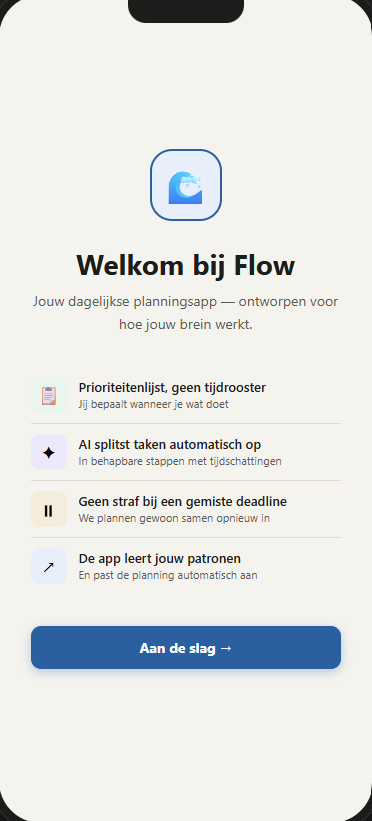
\includegraphics[width=0.38\linewidth]{introscherm.png}
\caption[Onboardingscherm]{Het onboardingscherm van Flow licht bij eerste gebruik
de vier kernprincipes toe: prioriteitenlijst, AI-taakverdeling,
niet-bestraffende herplanning en patroonherkenning.}
\label{fig:introscherm}
\end{figure}

De dagweergave is het startscherm van de applicatie. Bovenaan bevindt zich een
statistiekenbalk met het aantal taken van vandaag, het aantal dat aandacht
vereist en het totaal voor de lopende week. Taken worden weergegeven als
kleurgecodeerde kaarten gesorteerd op prioriteit. Een optionele tijdenknop
rechtsboven maakt het weekoverzicht bereikbaar voor wie een breder overzicht
wil.

\begin{figure}[h]
\centering
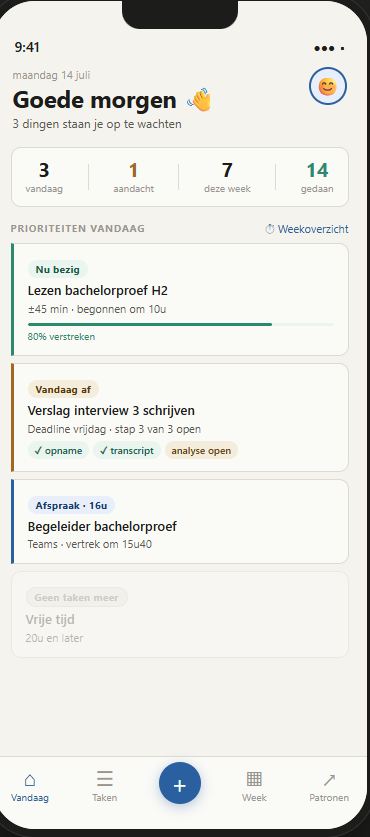
\includegraphics[width=0.38\linewidth]{dagoverzicht.png}
\caption[Dagweergave]{De dagweergave van Flow toont kleurgecodeerde taakkaarten
gesorteerd op prioriteit. Bovenaan staat een statistiekenbalk; rechts bevindt
zich een snelkoppeling naar het weekoverzicht.}
\label{fig:dagweergave-ontwerp}
\end{figure}

Wanneer een deadline niet gehaald wordt, toont de applicatie de volgende ochtend
een neutrale melding. Het herplanningsscherm biedt drie opties: de taak vandaag
inplannen, de taak heropdelen in kleinere delen, of de taak later in de week
inplannen. Onderaan staat een optie om de melding te negeren. Er verschijnen
geen rode tellers of cumulerende achterstanden.

\begin{figure}[h]
\centering
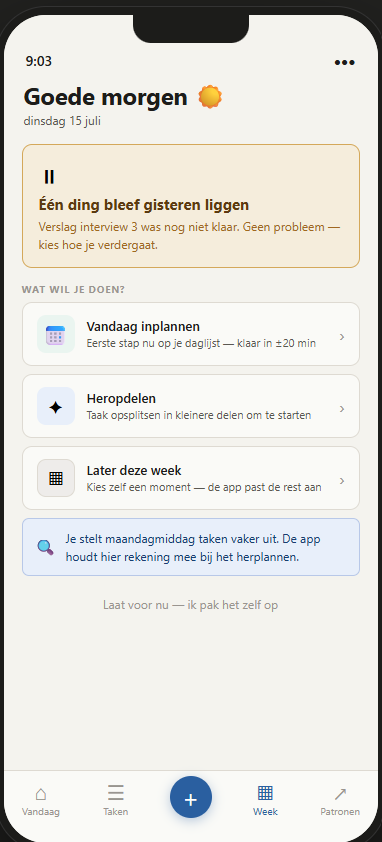
\includegraphics[width=0.38\linewidth]{gemistedeadline.png}
\caption[Herplanningsscherm]{Het herplanningsscherm toont een neutrale melding
bij een gemiste deadline. De drie herplanopties zijn: vandaag inplannen,
heropdelen, of later deze week. De term \textit{heropdelen} werd ingevoerd op
basis van feedback uit de open surveyantwoorden.}
\label{fig:gemiste-deadline}
\end{figure}

Het weekoverzicht toont een kalenderstrook van zeven dagen met gekleurde stipjes
per dag als visuele indicator van de taaklast. Eronder staan de taken per dag als
klikbare blokken. Dagen met een gemiste deadline worden afzonderlijk gemarkeerd.

\begin{figure}[h]
\centering
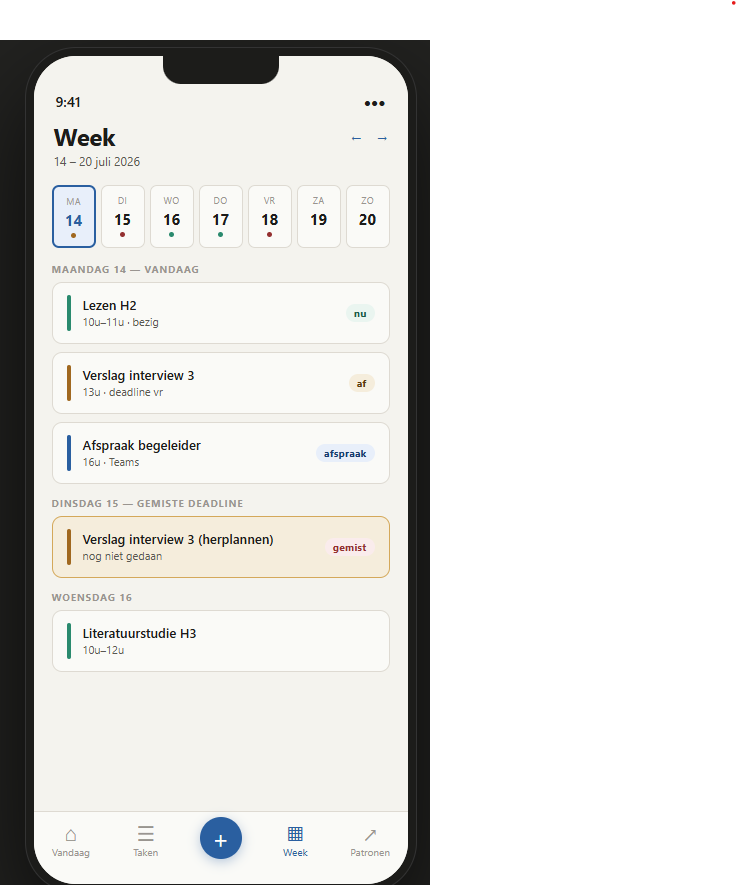
\includegraphics[width=0.38\linewidth]{weekoverzicht.png}
\caption[Weekoverzicht]{Het weekoverzicht biedt een kalenderstrook met
kleurstipjes per dag en klikbare taakblokken. Gemiste deadlines worden apart
gemarkeerd en leiden rechtstreeks naar het herplanningsscherm.}
\label{fig:weekoverzicht}
\end{figure}

De instellingenpagina groepeert de configuratie-opties in drie categorieën:
herinneringen (widget, dagelijkse melding, vertrekherinnering), weergave (thema,
dagweergavetype, AI-stappen) en planning (vrije blokken, patroonleren,
agenda-integratie). Agenda-integratie is de meest gevraagde ontbrekende
functionaliteit uit de open surveyantwoorden en is in de instellingen opgenomen
als toekomstige koppeling.

\begin{figure}[h]
\centering
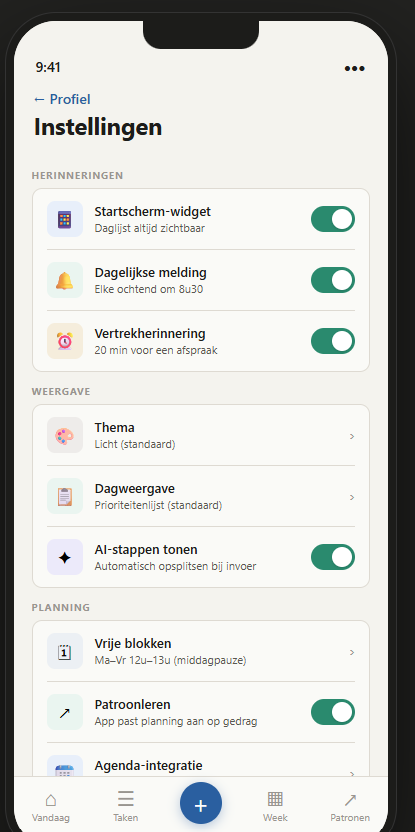
\includegraphics[width=0.38\linewidth]{instellingen.png}
\caption[Instellingenpagina]{De instellingenpagina groepeert opties in drie
categorieën. Agenda-integratie is opgenomen als configureerbare toekomstige
functionaliteit, op basis van de meest genoemde ontbrekende feature uit de
surveyresultaten.}
\label{fig:instellingen-ontwerp}
\end{figure}